%!TEX root = ../main.tex
%%%%%%%%%%%%%%%%%%%%%%%%%%%%%%%%%%
% Links:
%
% Difficulty: Companies: 
%%%%%%%%%%%%%%%%%%%%%%%%%%%%%%%%%%


%\begin{figure} \centering
%   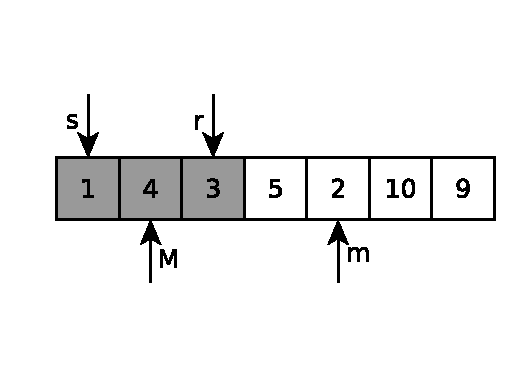
\includegraphics[width=\textwidth]{sources/max_num_chunks_sorted/images/example1}
%   \caption[Sample short cpation]{Sample Caption}. \label{fig:max_num_chunks_sorted:example1}
%   \end{figure}

\chapter{Sort the chunks, sort the array.}
\label{ch:max_num_chunks_sorted}
\section*{Introduction}
The problem asks for coutning the maximum number of subarrays we can split the array s.t. if we sort
each subarray individually then the whole arrays is sorted.

The idea is that you can greedily construct pieces of chuks from left to right. If the maximum of
the current chuck you are constructing is smaller than the minimum in the rest of the array, then
you can sort the chuck and no problem will arise because all the elements greater then the elements
in the chuck are further right and will be sorted later. This can be done with a set, where the set
keep tracks of the elements on the right and you can easily query for the minimum.



If the problem say that the elements are taken from the 0....n-1 (meaning that the array is a
permutation) then you can do this a bit better. 
\section{Problem statement}
\begin{exercise}
\label{example:max_num_chunks_sorted:exercice1}

	%example1
	\begin{example}
		\label{example:max_num_chunks_sorted:example1}
		\hfill \}
		
	\end{example}

	%example2
	\begin{example}
		\label{example:max_num_chunks_sorted:example2}
		\hfill \
		
	\end{example}

	\begin{example}
		\hfill \
	
	\label{ex:max_num_chunks_sorted:example1}
	\end{example}

	\begin{example}
		\hfill \

	\label{ex:max_num_chunks_sorted:example2}	
	\end{example}
\end{exercise}

\section{Clarification Questions}

\begin{QandA}
	\item 
	\begin{answered}
		\textit{}
	\end{answered}
	
\end{QandA}

\section{Discussion}
\label{max_num_chunks_sorted:sec:discussion}


\subsection{Brute-force}
\label{max_num_chunks_sorted:sec:bruteforce}

\begin{minipage}{\linewidth}
	\lstinputlisting[language=c++, caption={Sample Caption},label=list:max_num_chunks_sorted]{sources/max_num_chunks_sorted/max_num_chunks_sorted_solution1.cpp}
\end{minipage}

